% This must be in the first 5 lines to tell arXiv to use pdfLaTeX, which is strongly recommended.
\pdfoutput=1
% In particular, the hyperref package requires pdfLaTeX in order to break URLs across lines.

\documentclass[11pt]{article}

% Remove the "review" option to generate the final version.
\usepackage[review]{EMNLP2023}

% Standard package includes
\usepackage{times}
\usepackage{latexsym}

% New packages
\usepackage{lipsum}
\usepackage{booktabs}
\usepackage{mystyle}
\usepackage{multirow}

\newcommand{\system}{SysName}
\newcommand{\reading}{ReadName}
\newcommand{\planning}{PlanName}

% For proper rendering and hyphenation of words containing Latin characters (including in bib files)
\usepackage[T1]{fontenc}
% For Vietnamese characters
% \usepackage[T5]{fontenc}
% See https://www.latex-project.org/help/documentation/encguide.pdf for other character sets

% This assumes your files are encoded as UTF8
\usepackage[utf8]{inputenc}

% This is not strictly necessary, and may be commented out.
% However, it will improve the layout of the manuscript,
% and will typically save some space.
\usepackage{microtype}

% This is also not strictly necessary, and may be commented out.
% However, it will improve the aesthetics of text in
% the typewriter font.
\usepackage{inconsolata}

\usepackage{tabu}
\newsavebox{\DialogueBox}

\newenvironment{Dialogue}[1][\small]{
    #1
    \def\arraystretch{1.3}
    \setlength\tabcolsep{7pt}
    \taburulecolor{lightgray}
    \vspace{.8em}
    \noindent
    \begin{tabu} to \columnwidth {|[2pt]lX}
}{
    \end{tabu}
    \vspace{.5em}
}

\newcommand{\Partner}[1]{Partner: & \UserUtt{#1} \\}
\newcommand{\AgentDo}[1]{
\\[-1.3em]
\multicolumn{2}{|[2pt]p{\linewidth}}{ 
\AgentAction{#1}
}
\\[.3em]
}
\newcommand{\AgentSay}[1]{Agent: & \AgentUtt{#1} \\}
\newcommand{\UserUtt}[1]{\textit{#1}}
\newcommand{\AgentUtt}[1]{\textit{#1}}
\newcommand{\AgentAction}[1]{\texttt{\small #1}}
\newcommand{\MetaAction}[1]{\texttt{\small \underline{#1}}}
\newcommand{\Exec}{\MetaAction{\textcolor{red}{We don't use eval anymore!}}\xspace}
\newcommand{\Salient}{\MetaAction{refer}\xspace}
\newcommand{\Revise}{\MetaAction{revise}\xspace}
\newcommand{\ReviseConstraint}{\MetaAction{reviseConstraint}\xspace}
\newcommand{\Describe}{\MetaAction{describe}\xspace}
\newcommand{\scExec}{\texttt{\scriptsize\underline{eval}}\xspace}
\newcommand{\scSalient}{\texttt{\scriptsize\underline{refer}}\xspace}
\newcommand{\scRevise}{\texttt{\scriptsize\underline{revise}}\xspace}
\newcommand{\Recover}{\MetaAction{recover}\xspace}
\newcommand{\Root}{\textit{root}}
\newcommand{\OurDataset}{SMCalFlow\xspace}


\newcommand{\justin}[1]{{{\textcolor{purple}{(Justin: #1)}}}}
\newcommand{\derek}[1]{{{\textcolor{blue}{(Derek: #1)}}}}
\newcommand{\wenting}[1]{{{\textcolor{orange}{(Wenting: #1)}}}}
\newcommand{\daniel}[1]{{{\textcolor{brown}{(Daniel: #1)}}}}
\newcommand{\srush}[1]{{{\textcolor{green}{(Sasha: #1)}}}}


% If the title and author information does not fit in the area allocated, uncomment the following
%
%\setlength\titlebox{<dim>}
%
% and set <dim> to something 5cm or larger.

\title{
Integrating Symbolic Planning and Code Generation\\
for Grounded Dialogue
}

% Author information can be set in various styles:
% For several authors from the same institution:
% \author{Author 1 \and ... \and Author n \\
%         Address line \\ ... \\ Address line}
% if the names do not fit well on one line use
%         Author 1 \\ {\bf Author 2} \\ ... \\ {\bf Author n} \\
% For authors from different institutions:
% \author{Author 1 \\ Address line \\  ... \\ Address line
%         \And  ... \And
%         Author n \\ Address line \\ ... \\ Address line}
% To start a seperate ``row'' of authors use \AND, as in
% \author{Author 1 \\ Address line \\  ... \\ Address line
%         \AND
%         Author 2 \\ Address line \\ ... \\ Address line \And
%         Author 3 \\ Address line \\ ... \\ Address line}

\author{
Justin T. Chiu  \\
Cornell Tech \\
\texttt{jtc257@cornell.edu}
\And
Wenting Zhao \\
Cornell University \\
\texttt{wz346@cornell.edu}
\And
Derek Chen \\
Columbia University \\
\texttt{dc3761@columbia.edu}
\And
Alexander M. Rush \\
Cornell Tech \\
\texttt{arush@cornell.edu}
\And
Daniel Fried \\
Carnegie Mellon University \\
\texttt{dfried@cs.cmu.edu} 
}

\begin{document}
\maketitle
\begin{abstract}
Large language models (LLMs) excel at processing and generating text and code. However, LLMs have had limited applicability in grounded task-oriented dialogue as they are difficult to steer toward task objectives and fail to handle novel grounding. We present a modular and interpretable grounded dialogue system that addresses these shortcomings by composing LLMs with a symbolic planner and grounded code execution. Our system consists of a reader and planner: the reader leverages an LLM to convert partner utterances into executable code, calling functions that perform grounding. The translated code's output is stored to track dialogue state, while a symbolic planner determines the next appropriate response. We evaluate our system's performance on the demanding \textsc{OneCommon} dialogue task, involving collaborative reference resolution on abstract images of scattered dots. In this challenging setting, our system outperforms the previous state-of-the-art.
\end{abstract}

\section{Introduction}
% Dialogue needs planning
Success in grounded task-oriented dialogue requires intentional communication guided by strategic planning \citep{cicero}.
Dialogue agents must read partner utterances, update their beliefs, then make a plan that furthers their goal.
These plans must take into account both dialogue history and grounding, such as in an image.
In end-to-end systems based solely on large language models,
this process is implicit and therefore difficult to control,
requiring extra supervision \citep{rlhf} or expensive search \citep{astaresque} to improve.
While recent work has taken steps to rectify implicit reasoning via
planning in language space, 
where intermediate steps are generated by a language model \citep{cot},
there is no guarantee that these approaches result in strong plans.
Additionally, planning in language space is expensive,
requiring inference in a large language model.
\daniel{Relevance of CoT -- people may ask for a comparison to it? And will people know what language planning is?}

\begin{figure}[t!]
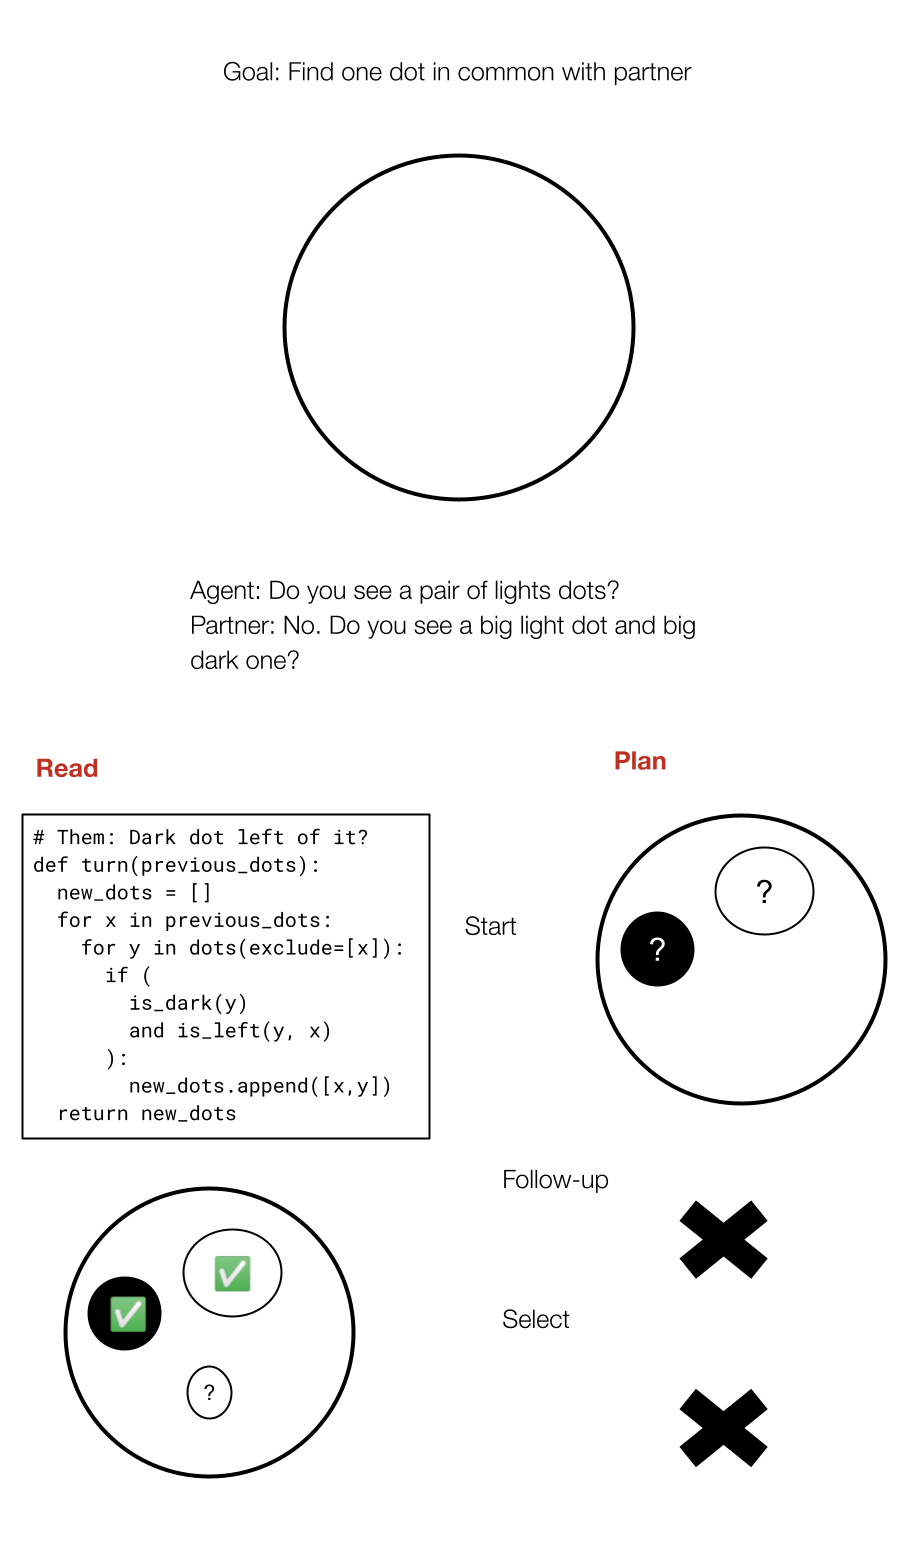
\includegraphics[width=\columnwidth]{imgs/Read-plan col.png}
\caption{
\label{fig:system}
System
}
\end{figure}

Rather than implicit or heuristic reasoning, we are interested in explicit reasoning and planning over
symbolic representations.
Symbolic representations are controllable by construction,
allowing system designers to easily build in task-specific knowledge \citep{he2018dnd,cicero}.
This controllability is crucial for obtaining task-specific success using general tools,
even with large language models.
% probably need examples here
%\justin{add in code}

We provide an example from \textsc{OneCommon}, 
a particularly challenging grounded dialogue game \citep{onecommon}.
The goal of \textsc{OneCommon} is to, through dialogue, identify and agree on one dot in common with your partner,
who has an overlapping but different view of an underlying set of dots, illustrated in Figure \ref{fig:system}.
Our symbolic representation is the set of dots mentioned in a particular utterance.
The difficulty in \textsc{OneCommon} is grounding the contextual spatial relationships described in language
to the visible dots, while ensuring that descriptions are not easily confused due to
the partner's different view.

\begin{comment}
There are three challenges in a dialogue system with symbolic representations:
1) scaling manually designed symbolic representations
2) mapping to and from symbols to language,
and 3) computationally reasoning over and composing those representations.
We build on recent work, which has shown that code-generating language models hold promise in addressing challenges 2 and 3, mapping to and from language as well as reasoning over symbols.
Promising results have been achieved in the visual question-answering and robotic instruction following domains
by using code-generating systems to map language to Python, leaving grounding to API libraries
that are called by the generated code \citep{vipergpt,codeaspolicies2022,gao2023pal}.
\daniel{I'm not sure this paragraph adds much, the intro is a bit long, and I don't know that we need to highlight the symbolic nature of the system -- just argue benefits of code directly. Maybe jump right into the next paragraph, and move these references there?}
\end{comment}

We utilize code-generation to map from language to symbolic rerpresentations.
Code-generation has a couple appealing properties:
First, it is well understood by large language models.
Modern language models are trained on a mixture of code and natural language, affording them the capability of, with some accuracy, translating between the two \citep{chen2021evaluating}.
Additionally, rather than mapping utterances directly to symbols and potentially utilizing shortcuts,
code acts as a compositional knowledge representation.
This allows for a code-generation system to potentially generalize to novel grounding,
provided a library of Python functions that perform the grounding for the system \citep{codeaspolicies2022}.

We present a system, \system{}, 
that reads by translating partner utterances into code,
uses the execution results to track dialogue state, and produces a symbolic plan of what to say next.
\system{} plans by optimizing expected information gain, which has been shown to be effective at building 
a key aspect of collaborative dialogue: common ground \citep{yu2019info,white-etal-2021-open,ocp}.
%\daniel{I think information gain is good to mention and will probably actually be more familiar to an NLP audience than ``partner model.'' Maybe reorder these two concepts?}

We evaluate \system{} on \textsc{OneCommon},
a grounded dialogue task where the given human demonstrations are often suboptimal and the visual grounding
is out-of-domain for vision models.
\daniel{maybe telegraph these as benefits of code earlier, if you don't already}
\justin{does this come out better in the previous paragraph?}
Our goal is to out-perform human demonstrations on the hardest setting
with a minimally supervised approach.
We show that \system{} accomplishes this both in human evaluation as well as selfplay,
demonstrating the effectiveness of planning with code-generation as glue.

\section{Related work}
Dialogue systems have a long history of reasoning with symbolic representations.
%In 1968, \citet{winograd} developed the SHRDLU system, which was a rule-based grounded dialogue systemthat discussed a simple block world with a partner.
When available, symbolic representations have been found to improve
the performance of dialogue systems, especially in the setting of grounded dialogue games \citep{winograd,young2006pomdp,he2018dnd,cicero}.
\textsc{Cicero} in particular utilizes symbolic planning in a \textsc{Diplomacy} system,
a strategy game that requires negotiation and possibly deception \citep{cicero}.
\textsc{Cicero} requires a supervised dataset for training their system.
We utilize code-generating large-language models for minimial supervision, but require a hand-crafted perception API.
Prior work in symbolic reasoning for dialogue also painstakingly crafts domain-specific executable representations  and composition operators \citep{sm}.
We show that, in order to deal with novel grounding, code generation and planning with symbolic representations
are effective.
We utilize Python for grounding utterances in context and avoid designing a domain-specific language.

Planning in dialogue systems has recently eschewed symbolic representations in favor of
planning directly in text, 
where systems either perform roll-outs, tree-search, or other forms of intermediate reasoning in language.
This allows system designers to avoid manually defining symbolic representations \citep{yarats2017rollout,jang2020bapomdp,gandhi2023strategic}.
However, the accuracy of language-space planners is still low in many settings \citep{valmeekam2023planning}.
We focus on symbolic planning, where planning is defined in a narrow space that is correct and controllable by construction.

With the recent progress in large language modeling,
code generation for modular grounded systems has quickly gained interest.
They do not require task-specific training data, relying solely on large pretraining for generalization, API definitions for grounding, and a few usage examples for contextualization,
making them cheap to apply.
A body of work utilizes a large language model for instruction following
by generating Python code that makes calls to lower-level perception libraries
\citep{codeaspolicies2022,vipergpt,gupta2022visual,gao2023pal}.
This extends prior work on executable semantic parsing \citep{liang2016learning,johnson2017inferring,cheng2018learning} with large language models.
We apply these advances to the setting of grounded dialogue,
where code generation grounds language to a novel visual context for use in
explicit planning in dialogue system \citep{young2013pomdpsurvey}.

Prior work on collaborative reference games focus on building common ground
\citep{mf,pb,pip}.
Prior work by \citet{fried} implements an approximation of pragmatic reasoning on \textsc{OneCommon}, but plans in language space and utilizes supervised models for mapping language to symbols.
\citet{pip} plan in symbolic space, but do not incorporate natural language. 
We plan in symbolic space and map from language to symbols via code generation.

\section{Problem setup: Reference games}
This section describes the problem setup of collaborative reference games, a type of collaborative dialogue.

We focus on collaborative reference games, which
pair an agent and a partner in order to agree on a shared object through natural language dialogue \citep{pb,pip,mf,onecommon}.
Mirroring realistic scenarios, many reference games are also partially observable,
where the agent and partner have different perspectives, and so they must resolve ambiguity by building common ground.

% notation
At each turn, the agent \textbf{reads} the partner's utterance, converting it into a symbolic representation, $y$.
The agent \textbf{plans} by updating its symbolic representation of the dialogue state, $z$, given $y$,
then reasoning about what to say next, producing their own symbolic plan, $x$.
We illustrate this process in Figure \ref{fig:setup}.
\justin{todo figure with mapping to and from language / planning in symbol space}

As a representative reference game, we study \textsc{OneCommon}.
In \textsc{OneCommon}, the agent and partner see different but overlapping views of a set of dots, and the goal is to find one dot in common.
\textsc{OneCommon} is particularly difficult due to its partial observability and visual context,
illustrated in Figure \ref{fig:oc}.
The visual grounding in \textsc{OneCommon} was constructed to make referring expressions ambiguous, with continuous-valued sizes, colors, and positions of dots \citep{onecommon}.

A natural symbolic representation for both partners and agents, $y$ and $x$ respectively, in reference games is the set of objects mentioned.
In \textsc{OneCommon}, this takes the form of sets of dots to ask about, as well as any answers to previous questions.

\section{Reading: From language to symbols}
%\justin{title is kind of a waste, need to connect to decode / encode story}
Our approach to grounded reference games separates symbolic reasoning from language, allowing explicit steering.
%As the goal of reference games is to reason about shared objects, a set of objects is a natural symbolic representation.
%Given this representation, reading consists of mapping from utterances to the set of objects that are mentioned, and planning means reasoning about the most useful objects to ask about next.
Reading consists of mapping from utterances to symbolic representations, and planning reasons about what to ask next in symbolic space.

We address three challenges in reading: First, reading requires grounding utterances in context. Second, utterances are compositional. Utterances build on top of each other, while each individual utterances themselves consists of smaller semantic components. Third, systems must solve the previous two challenges quickly, as real-time dialogue systems require reasonable response times.

We illustrate these challenges with an example from \textsc{OneCommon}.
Systems must be able to understand exchanges such as 

\begin{Dialogue}
    \AgentSay{Do you see a triangle?}
    \Partner{Yes, next to a small grey dot.}
\end{Dialogue}%

\noindent where spatial relationships are described compositionally,
building upon each other.

Our system, \system{}, reads partner utterances by generating and executing code.
Code is a fitting semantic representation of grounded dialogue
with compositional structure,
naturally mirroring the ability of referring expressions to
refer to and build upon previous utterances.

Given an utterance, we generate a code representation of that utterance, a function that yields the partner's symbolic representation, $y$.
The code representation consists of a series of perceptual library functions with grounded semantics, drawn from a predefined API.
This API allows the system to decompose complex grounding into step-by-step reasoning.
We provide an example of a code representation in \textsc{OneCommon} below:

\begin{Dialogue}
    \AgentSay{Do you see a triangle?}
    \AgentDo{agent\_plan\_x = [[a,b,c]]}
    \Partner{Yes, next to a small grey dot.}
    \AgentDo{%
      def turn(prev\_mentions):\newline
      \strut~~mentions = set()\newline
      \strut~~for a,b,c in prev\_mentions:\newline
      \strut~~~~for d in single\_dots():\newline
      \strut~~~~~~if (\newline
      \strut~~~~~~~~is\_small(d)\newline
      \strut~~~~~~~~and is\_grey(d)\newline
      \strut~~~~~~~~and all\_close([a,b,c,d])\newline
      \strut~~~~~~):\newline
      \strut~~~~~~~~mentions.add([a,b,c,d])\newline
      \strut~~return mentions\newline
      partner\_mentions\_m = turn(agent\_plan\_x)
    }
\end{Dialogue}%

\noindent 
The perceptual library functions, \texttt{is\_small}, \texttt{is\_grey}, and \texttt{is\_close}, are drawn from a manually-defined library.
For \textsc{OneCommon}, we define these functions using domain-specific knowledge:

\begin{Dialogue}
\AgentDo{
def is\_small(d): return d.size < -0.3
}
\end{Dialogue}

\noindent We provide the full library for \textsc{OneCommon} in Appendix \ref{sec:library}.

We utilize the code-generating abilities of large language models to generate the code representations of utterances.
While LLMs are capable of generating entire code representations in a single prompt, the outputs are long.
Long outputs result in a system that is too slow for real-time grounded dialogue.
Practically, our system must therefore break down generation into a series of steps in order to reduce output length and increase execution speed.
We give an example of one such decomposition for \textsc{OneCommon}:

\textbf{Dialogue act} First, we classify partner utterances as one of three dialogue acts:
The \textsc{start} of a new line of questions, a \textsc{follow-up} question, or a signal to end the game.

\textbf{Refer} Second, given the dialogue act, we predict which turn the utterance is following up on, if any.
For example, 

\begin{Dialogue}
    \AgentSay{Do you see a triangle?}
    \Partner{Yes, next to a small grey dot.}
    \AgentDo{%
        dialogue act: \textsc{follow-up}\newline
        refer: turn 1
    }
\end{Dialogue}%

\noindent The system is then able to infer the dots mentioned in the previous turn: \texttt{a,b,c}.

\textbf{Fragment generation} Third, we predict the number of new dots mentioned in the partner utterance alongside code fragments that express the semantics -- without the boilerplate code in the example above:

\begin{Dialogue}
    \Partner{Yes, next to a small grey dot.}
    \AgentDo{%
      1 new dot\newline
      is\_small(d)\newline
      is\_grey(d)\newline
      all\_close([a,b,c,d])
    }
\end{Dialogue}%

\textbf{Stitch} Finally, we utilize a template to stitch all of this information back into the full code representation for execution.

\section{Symbolic planning}
The goal of collaborative reference games is to build common ground quickly and accurately.
This requires solving two challenges: careful reasoning about what information has been gathered so far, as well as what to say next.
Our system, \system{}, addresses both of these by planning in symbolic space,
utilizing the symbolic representations produced by reading.

We rely on a framework known as optimal experimental design, where agents reason probabilistically and choose the most informative plan by relying on a model of partner responses \citep{lindley,chaloner,dp}.
Under this framework, the agent starts every turn with a prior belief over possible symbolic states, $p(z)$. The agent reads the previous partner utterance, obtaining the symbolic representation, $y$, to the agent's previous plan, $x$, then updates that belief recursively.
This update relies on a partner model $p(y|x,z)$,
which predicts the partner's symbolic response given state $z$ and plan $x$.

Something about grounded models here, mentioning symbolic space.

The belief update is then given by:
\begin{equation}
\label{eqn:update}
p'(z) = p(z \mid x, y)
= \frac{p(y \mid x,z)p(z)}{\sum_z p(y\mid x,z)p(z)}.
\end{equation}
Taking this posterior distribution to be our updated belief, $p'(z)$, the agent then decides whether to propose a new plan or signal to end the game.

As the goal of reference games is to find a shared object, we utilize the following stopping rule: if the probability of any object is greater than hyperparameter $\theta$, select that object.

Otherwise, the agent finds a new plan by optimizing expected information gain \citep{lindley}:
\begin{equation}
\label{eqn:eig}
\argmax_x H[z] - \Es{y \mid x}{H[z \mid x,y]},
\end{equation}
where $H[z]$ is the entropy of the updated belief $p'(z)$\footnote{The belief entropy $H[z]$ in the definition of information gain is constant with respect to
the plan $x$, and can be dropped from the objective.}
and $H[z\mid x,y]$ the posterior after receiving imagined response $y$ to proposed plan $x$.



\section{Experimental setup}
We conduct two experiments,
evaluating \system{} on the \textsc{OneCommon} task.
First, we perform human evaluation, evaluating how successful systems are when paired with unconstrained human partners who utilize linguistically diverse utterances and a range of strategies.
Second, we perform selfplay, pairing systems with a copy of themselves to isolate strategic efficiency.

\textbf{Hyperparameters}
Throughout, \system{} uses a belief threshold hyperparameter $\theta = 0.8$
and GPT-4\footnote{Specifically \texttt{gpt-4-0613}.} for reading \citep{gpt4}.

\textbf{Parameterization}
The belief over symbolic states, $p(z)$,
captures which dots are shared in \textsc{OneCommon}.
We utilize a globally normalized model over all sets of dots,
scoring each set based on the minimum spanning tree
whose edge weights are determined by the rank of how close neighboring dots are.
The partner 
We additionally utilize the minimum spanning tree to constrain the response model, $p(y|x,z)$.
The details of both models given in Appendix \ref{sec:parameterization}.

\textbf{Baseline} We compare to the state-of-the-art baseline system of \citet{fried},

\section{Experiments}
This section reports the primary evaluations in \textsc{OneCommon}:
human evaluation and selfplay.

\textbf{Human evaluation}
Our primary evaluation is
human evaluation in \textsc{OneCommon} dataset \citep{onecommon},
which measures game success with human partners.
\system{} outperforms the baseline model of \citet{fried},
but does not exceed human performance.

\begin{table}[!t]
\centering
\begin{tabular}{lrrr}
\toprule
Agent                   & Success & Turns & Games\\
\midrule
\system{}               & 67.0\%  & 7.77 & 117\\
\citet{fried}           & 56.5\%  & 6.66 & 96\\
Human                   & 80.0\%  & 6.05 & 67\\
\quad - expert          & 65.4\%  & 6.07 & 26\\
\quad w/ expert         & 90.2\%  & 6.05 & 41\\
\hline
Human$^\dagger$         & 65.8\%  & 4.97\\
\bottomrule
\end{tabular}
\caption{\label{tbl:human-eval}
The success rate of different agents with human partners on the hardest setting of \textsc{OneCommon}, with 4 shared dots.
A higher success rate is better.
$^\dagger$ indicates the performance is from the \textsc{OneCommon} dataset
\citep{onecommon}.
}
\end{table}

\subsection{Selfplay}
We also report success in selfplay, where agents play with a copy of themselves.
While selfplay only gives an imperfect proxy for how a system will perform with human partners, it eliminates the variance of human evaluations that is due to e.g., linguistic and partner skill diversity.

Speculative: \system{} outperforms the original human performance in
the \textsc{OneCommon} dataset,
where humans were coached in order to improve data quality \citep{onecommon}
(also cite personal communication with Udagawa).
Speculative: \system{} takes more turns on average, but
has a higher success rate.
We hypothesize that this is caused by shorter human partner
responses to the system.
The average number of words per utterance when playing with \system{} is \justin{XX},
as opposed to \justin{YY} when partnered with another human.

\textbf{Systems}
For selfplay, we consider a wider variety of systems than human evaluation, due the reduced cost of evaluation.
We compare \system{} to RNN \citep{fried},
a prompt-based text-only language model baseline,
ViperGPT \citep{vipergpt},
and BLIP2 \citep{blip2}.

\begin{table}[!t]
\centering
\begin{tabular}{lrr}
\toprule
Agent                   & Success & Avg \# turns\\
\midrule
\system{}$$             & 84.0\% & 4.83\\
\citet{fried}           & 63.5\%  & 3.31\\
%GPT4                    & \%      & \\
%ViperGPT                &         & \\
\hline
Human$^\dagger$         & 65.8\%  & 4.97\\
\bottomrule
\end{tabular}
\caption{\label{tbl:selfplay}
The success rate of different agents in 200 selfplay games on the hardest setting of \textsc{OneCommon}, with 4 shared dots.
A higher success rate is better.
The human performance is from the \textsc{OneCommon} dataset
\citep{onecommon}.
}
\end{table}

A similar pattern from human evaluation holds in selfplay,
where \system{} outperforms all other systems and humans.
Additionally, the results from reference resolution are also reflected in selfplay,
as ViperGPT and BLIP2 have low success rates due to grounding errors.

The average number of turns per game of \system{} is more comparable 
to the average for human-human games, likely due to \system{}
being constrained to ask a new question at every turn.

\section{Analysis}
This section presents further analysis on planning, prompting for code generation, and reference resolution.

\subsection{Human evaluation analysis}

\begin{table}[!t]
\centering
\begin{tabular}{lr}
\toprule
Agent                    & Avg partner utt len\\
\midrule
\system{}                &  6.95 \\
\citet{fried}            & 9.62  \\
Human                    & 15.06  \\
\bottomrule
\end{tabular}
\caption{\label{tbl:refres}
Average partner utterance length for different systems in human evaluation.
}\end{table}




\subsection{Plan analysis}
We present qualitative examples of plans generated by \system{}, as well as \citet{fried} in Figure \ref{fig:plans}.
We explore two settings: The first is.
The second is.

As \system{} performs symbolic belief updates and directly optimizes information gain,
the system is more responsive and cohesive, compared to the model from prior work \citep{fried}.
In the all-yes setting, \system{} does X, whereas the baseline does Y.
In the alternating setting, \system{} does X, whereas the baseline does Y.

\subsection{Prompt analysis}
We explore different prompting styles for reading in \system{}.
\system{} uses a sequence of two prompts for parsing plans:
the dialogue act and new dots are classified,
then code fragments.
Those fragments fill in a templated Python function,
which is then given an argument based on a backpointing heuristic.
\daniel{need to say more about ``backpointing heuristic''}
We explore an alternative method of prompting, that prompts
a code-generating system to directly produce the final Python function,
as well as the backpointer, in a single prompt


We present the results on reference resolution,
employing the same template generations from Section \ref{sec:refres}.

\begin{table}[!t]
\centering
\begin{tabular}{lrrr}
\toprule
Prompt style                   & Acc     & Time (s) & Len\\
\midrule
\system{}                      & 57/75  & 10    &  234\\
Single prompt                  & 63/75  & 48    &    \\
\bottomrule
\end{tabular}
\caption{\label{tbl:prompt}
An analysis of different code generation prompt styles.
}
\end{table}

In Table \ref{tbl:prompt}, we see that the two prompting styles achieve similar accuracy, but have a large difference in time as well as output length.
The single prompt system must contain the generated code for every utterance, including agent utterances.
This was avoided in \system{}, resulting in large slowdowns.

\textbf{Ideally use other systems too}
gpt 3.5, bard, starcoder?
\daniel{Maybe starcoder if it isn't terrible, but I don't see much advantage to having two proprietary systems}


\subsection{Reference resolution}
\label{sec:refres}
We first conduct a preliminary study on generalization in reference resolution, validating our approach to reading.
We evaluate whether different systems are able to accurately understand templated descriptions of pairs of dots, providing an upper bound on the generalization ability of reference resolution systems.
A system that is unable to resolve references to pairs of dots is unlikely to generalize to more complex configurations.
%\daniel{Can you motivate why we do this rather than use human-written language?}
Template generations take two dots, chosen as a plan from \system{},
and describes the sizes and colors of those two dots, as well as the relative positions.
For this evaluation alone, the resolution system has the same view as the partner,
a departure from the standard partial overlap setting in \textsc{OneCommon}.
We report the exact match accuracy of the resolved plan for 25 examples.
\justin{for now, will extend. also have results for follow-up + select.}

\textbf{Systems}
We compare \system{} to ViperGPT, a visual grounding system that uses code as a representation \citep{vipergpt},
\daniel{I'd describe this as a visual grounding system that uses code as representation, or describe ViperGPT and BLIP2 as both strong VQA systems, one of which uses code as a representation}
BLIP2, a strong visual question-answering and captioning system \citep{blip2},
and the previous state of the art for \textsc{OneCommon} RNN \citep{fried}.

\begin{table}[!t]
\centering
\begin{tabular}{lr}
\toprule
Agent                    & Acc\\
\midrule
\system{}                &  23/25 \\
GPT4-MC                  & \%  \\
\citet{fried}            & 4/25  \\
BLIP2                    & \%  \\
\bottomrule
\end{tabular}
\caption{\label{tbl:refres}
Reference resolution accuracy on template generations.
}
\end{table}

We find that vision-based models as well as 
language-only models are much less accurate than
our code-based grounding approach for this task,
shown in Table \ref{tbl:refres}.
We hypothesize that this is due the visual context in \textsc{OneCommon} being to out-of-domain for most image models.
We also find that the previous state-of-the-art approach,
RNN \citep{fried}, has difficulty recognizing simple utterances.
We hypothesize that this is also caused by distribution shift:
the reference resolution model of RNN captures both
language descriptions as well as the distribution of dots
preferred by the human demonstrations it was trained on,
resulting in failure to generalize to simple 2-dot combinations.
The code-generation approach does not have this issue,
as it only captures information in the utterance
rather than what dots were described during training.
\daniel{This makes it sound like we're testing our system on easier examples than we'd actually get from people. Are the plans you use here chosen from a fairly unconstrained set? if so, can you emphasize this being the source of the generalization, rather than the plans being simpler?}

\section{Conclusion}
\justin{TBD}
%\section{Conclusion}
%TBD

\section*{Acknowledgements}
Vivian Chen, Ge Gao, Omer Gul, Sedrick Keh, Woojeong Kim, Celine Lee, Jack Morris, Chenran Ning, Jacob Sharf, Alane Suhr, Nicholas Tomlin, Anne Wu, Jiawei Zhou.

\section*{Limitations}
There is a tradeoff between expressivity and  controllability for dialogue partner modeling.
In this work, we emphasize controllability by explicitly modeling certain aspects of the partner perspective while not accounting for others, resulting in biased agents.
The failure to account for
particular partner aspects may affect fairness and equity with a diverse pool of partners.

%\section*{Ethics Statement}

% Entries for the entire Anthology, followed by custom entries
\bibliography{anthology,custom}
\bibliographystyle{acl_natbib}

\appendix

\subsection{Symbolic planning with information gain}
\justin{take out of bckgurnd and put to meth}
A common framework for approximately solving reference games is information gain, otherwise known as optimal experimental design, where agents choose the most informative action \citep{lindley,chaloner,dp}.
This framework has been utilized in recent works on multi-turn, asymmetric reference games similar to 20 questions or \textsc{Guess Who?},
where the agent is restricted to asking questions and the partner to answering \citep{yu2019info,white-etal-2021-open,rao2018q}.
%\daniel{Consider using a different term rather than ``optimal experiment design'' to follow the NLP papers above, and maybe say it's like 20 questions}
In this section, we describe its application to collaborative reference games, where both the agent and partner are unrestricted.

Every turn, the agent starts with a belief over which objects are shared, $p(z)$, where each $z$ is a set of objects. The agent reads the previous partner utterance to resolve what objects they mentioned, $o$, as well as any responses, $y$, to previous agent mentions $x$.
The agent then plans by finding the set of objects to describe that is most informative about what objects are shared.

\textbf{Belief update} 
Given objects the partner mentioned, $o$, the agent updates their belief over shared objects:
\begin{equation}
\label{eqn:update-mention}
p(z \mid o)
= \frac{p(o | z)p(z)}{\sum_z p(o | z)p(z)},
\end{equation}
filtering out shared states $z$ that do not contain the mentioned objects.

The partner may also respond to agent mentions described in the preceding turn, resulting in a similar belief update.
We denote the agent's mentions as $x$, and the partner's response as $y$:
\begin{equation}
\label{eqn:update}
p(z \mid x, y)
= \frac{p(y \mid x,z)p(z)}{\sum_z p(y\mid x,z)p(z)},    
\end{equation}
upweighting states $z$ where the response $y$ is likely under the partner response model $p(y|x,z)$.

\textbf{Planning} The belief update gives us a new belief which is then used for planning.
Planning finds the agent mentions that maximize the expected information gain \citep{lindley} about belief $z$,
\begin{equation}
\label{eqn:eig}
\argmax_x H[z] - \Es{y \mid x}{H[z \mid x,y]},
\end{equation}
where $H[z]$ is the entropy of the belief\footnote{The belief entropy $H[z]$ in the definition of information gain is constant with respect to
the plan $x$, and can be dropped from the objective.}
 and $H[z\mid x,y]$ the posterior after receiving response $y$ to mention $x$.

\textbf{Selection} After gathering information through planning and
incorporating information through belief updates,
the agent must decide when it has built enough common ground via a stopping rule,
collaboratively selecting a shared object with its partner.
Stopping rules can be solved exactly via dynamic programming or implemented heuristically.
%\daniel{how does it decide?}

\section{Method}
Our approach to reference games follows the expected information gain framework.
Our system, \system{}, separates symbolic plans from language,
allowing explicit steering.
As the goal of \textsc{OneCommon} is to reason about shared dots,
a set of dots is a natural plan representation.
Given this representation, reading consists of mapping from utterances to the set of dots that are mentioned, and planning means finding the set of dots to ask about next via information gain.
\justin{Need to link back to contributions: top-down implies contribution down}
\justin{too much structure. no hopping from text to examples}

\subsection{Reading as code generation}
The goal of reading in \system{} is to obtain a symbolic representation of an utterance, which can then be used in planning.
In \textsc{OneCommon}, we need to resolve sets of dots that are mentioned both explicitly and implicitly. For example, the partner's utterance in

\begin{Dialogue}
    \AgentSay{Do you see a triangle?}
    \Partner{$\underbrace{\text{Yes}}_{\text{\normalfont response}}$, $\underbrace{\text{next to a small grey dot}}_{\text{\normalfont mention}}$.}
\end{Dialogue}%

\noindent mentions all dots in the triangle as well as the small grey dot, even though the triangle was elided and not explicitly mentioned.
Additionally, \system{} must also understand responses to previous agent mentions, e.g. the `Yes' in the above example.

\system{} accomplishes this via a 3-step process:
Partner responses are classified, 
the system predicts the dialogue act of the partner utterance,
and finally, a code representation of the utterance given the dialogue act.
We make the simplifying assumption that the responses are binary \textsc{yes}/\textsc{no}, and consider 3 coarse dialogue acts related to referring expressions:
the \textsc{start} of a line of questioning,
\textsc{follow-up} questions that continue a line of questioning,
and finally \textsc{select} an object.

\textbf{Code generation}
Mentions are resolved by translating utterances into code, then executing that code.
The code is intended to express and execute the underlying task-specific semantics of an utterance.
%\justin{Why code? handle novel grounding and easily compose with previous mentions}
Code allows the system to handle novel grounding, given a suitable underlying base library of functions,
as well as easily compose the current utterance's meaning with previous turns.

Following Code-as-Policies \citep{codeaspolicies2022},
code generation relies on a base library and a code-generating language model.
We design a library of 40 constraint functions that cover dot sizes and colors, as well as spatial relationships between dots such as \texttt{is\_left}, \texttt{is\_triangle}, and \texttt{is\_close}. We provide all functions and their implementations in Appendix \ref{} or supplementary material.

We provide examples of generated code for utterances corresponding to each dialogue act below.

\textbf{Example: \textsc{start}} Our first example is \textsc{start}:

\begin{Dialogue}
    \Partner{Do you see a black dot?}
    \AgentDo{%
      def turn(state):\newline
      \strut~~state = set()\newline
      \strut~~for a in single\_dots():\newline
      \strut~~~~if is\_dark(a): state.add([a])\newline
      \strut~~return state
    }
\end{Dialogue}%

\noindent The function loops over all individual dots, returned by the
\texttt{single\_dots()}, and returns the set of all singleton dark dots.
As a convention, the \texttt{turn} function also takes a \texttt{state} argument,
which is used to build on the results of previous turns.
We will see an example of this in the next example.
As this is a \textsc{start} utterance, the argument \texttt{state} is not used.

\textbf{Example: \textsc{Follow-up}} Next, we have

\begin{Dialogue}
    \Partner{Do you see a big black dot?}
    \AgentSay{Yes, next to a small grey dot.}
    \Partner{I don't see that, but is there a light dot to the left of the black one?}
    \AgentDo{%
      def turn(state):\newline
      \strut~~for a, in state:\newline
      \strut~~~~for b in single\_dots():\newline
      \strut~~~~~~if (\newline
      \strut~~~~~~~~is\_light(b)\newline
      \strut~~~~~~~~and is\_left(b, a)\newline
      \strut~~~~~~~~and is\_dark(a)\newline
      \strut~~~~~~):\newline
      \strut~~~~~~~~state.add([a,b])\newline
      \strut~~return state
    }
\end{Dialogue}%

\noindent This utterance denies the plan of the previous turn 
and instead builds upon the plan from the first turn, adding a new dot.
As a result, when executing this function,
we must resolve the correct value of \texttt{state} to pass in, the output of a previous turn.
Similar to \citet{sm}, we utilize a task-specific heuristic for resolving \texttt{state}.
We define \texttt{state} as the set of dots considered in the last confirmed turn,
a naive form of backtracking. We also present experiments that use a large language model to predict backpointers in Section \ref{sec:experiments}.

\textbf{Example: \textsc{Select}} Lastly, we give an example of a \textsc{select} utterance,
which communicates an intent to end the game.

\begin{Dialogue}
    \Partner{Do you see a big black dot?}
    \AgentSay{Yes, next to a small grey dot.}
    \Partner{Let's select the small one.}
    \AgentDo{%
      def turn(state):\newline
      \strut~~for a,b in state:\newline
      \strut~~~~~~if is\_small(dot)): state.add([b])\newline
      \strut~~return state
    }
\end{Dialogue}%

\noindent The \textsc{turn} function of a \textsc{select} utterance filters the state down to a list of single dots, the candidates for selection.


\textbf{Prompting}
We implement each step of reading using few-shot prompting with large language models, which has shown effective for semantic parsing \citep{shin-etal-2021-constrained}.
Partner utterance response classification and dialogue act classification both utilize few-shot prompts.
The dialogue act classification prompt additionally predicts the number of new dots mentioned for 
\textsc{start} and \textsc{follow-up} utterances, as well as the selected dot for \textsc{select} utterances. This aids in subsequent code generation.

Given the dialogue act,
we translate utterances such as ``Do you see a big black dot'' into a series of constraints expressed as Python functions:

\begin{Dialogue}
    \Partner{Do you see a big black dot next to a light one?}
    \AgentDo{%
      2 new dots\newline
      is\_dark(a)\newline
      is\_large(a)\newline
      is\_light(b)
    }
\end{Dialogue}%

\noindent Given these code fragments, we use a template to 
construct the full \texttt{turn} function shown in the examples above.
\justin{say how this is done (template)}


\subsection{Symbolic planning}
After reading, the agent updates its belief then plans what to say next.
\justin{Chronological is bad. second part of the module is understanding what to say, in this way. give motivations and objectives. what part of process it has to handle. need to setup the goals and accomplish them, link back to contribs}

In each turn, the agent can update its belief over shared objects twice after reading.
First, if the partner responded to the agent's last plan,
and second, if the partner mentioned a plan that the agent sees.
In the first case, the belief update simply follows Equation \ref{eqn:update}.
In the second case, the belief update is similar, but the agent only updates their belief if the agent response is \textsc{yes}.

Once updated, the new belief is used to construct the agent's next plan.
The agent first decides whether to confirm or deny the dots in the partner plan,
then chooses the dialogue act and the agent's own dot plan jointly.
The choice of dot plan follows the optimal experiment design framework 
in Equation \ref{eqn:eig}, with some modifications.

Ideally, the agent would optimize an objective based on both information gain and communicative cost or surprisal.
Rather than directly optimize such an objective,
we instead introduce task-specific constraints on dot plans and optimize information gain under those constraints.


We choose between dialogue acts, \textsc{start}, \textsc{follow-up}, and \textsc{select}, based on informativity and the probability of successful coordination. If a dot is shared with probability above a belief threshold hyperparameter, $\theta$, the agent chooses to \textsc{select}.
Otherwise, the agent chooses to \textsc{start} asking about 
new dots or a \textsc{follow-up} question
about an existing set based on the expected information gain.
We heuristically encode communication cost by constraining \textsc{start} questions to only ask about at most two dots, and \textsc{follow-up} questions
to ask about a single new dot.

\textbf{Parameterization}
We build on the prior and partner model proposed by \citet{ocp},
who utilize a uniform prior over shared objects, $p(z)$,
and a response model $p(y|x,z)$ that takes into account the partner's
unobserved perspective.

We extend their approach by proposing a globally normalized model over the powerset of dots
that takes into account how close dots are together.
Each subset of dots is scored based on a minimum spanning tree,
whose weights are determined by how close dots are.
We additionally utilize the minimum spanning tree to constrain the response model, $p(y|x,z)$.
The details of both models given in Appendix \ref{sec:parameterization}.

%Generation
\textbf{Writing}
Plans are described using rule-based templates.
Writing uses one simple template for each of the three dialogue acts,
given in Appendix \ref{sec:templates}.
In practice, this could be extended to more flexible albeit higher latency response generation.


%\section{Templated generation}
%\label{sec:generation}
%TBD

\section{Blah}
\textbf{Belief state and response model}
The agent maintains a belief distribution over which of the 7
dots are shared, represented as a distribution over boolean vectors of size 7.
Maintaining and updating this belief distribution requires both a prior over shared dots
and a response model.

We utilize a globally normalized prior over boolean vectors.
The prior's energy function is derived from the minimum spanning tree of the shared dots, where the weights of edges are determined by the ranking of how close dots are and the score of a tree is the sum of the weights of edges.
We provide details in Appendix \ref{sec:prior}.
We use the response model from \citep{ocp}, which explicitly accounts for perspective dependent ambiguity
by including a confusion model that accounts for the partner mis-resolving dots due to differences in perspective.


\section{Partner Modeling in Reference Games}
\label{sec:planning}

Collaborative reference games pair an agent and a partner in order to agree on a shared object through natural language dialogue.
At each turn, the agent or partner may decide to terminate the game and make a selection.
Once either the agent or their partner terminates, the other player must also act (without observing the other's choice). If both agent and partner agree, both win; otherwise, both fail. 

Our approach to reference games separates planning of utterances (choosing what to talk about) from surface realization (choosing how to say it).
At each turn, our agent produces an utterance plan $x$ by using a \emph{partner model}, which simulates the partner's possible responses, $y$, given their hidden perspective, $z$.
The agent uses the partner model to infer the partner's perspective and predict the partner's responses to the agent's plans.
We first give an overview of the partner model 
and planning procedure in this section.

% restate goal and contribution
\noindent \textbf{Partner model}
We model the partner's perspective as a latent variable, infer the value for this variable over the course of a game, and use it to plan generation.
This contrasts with a typical egocentric heuristic, as used in \citet{fried}, which assumes the partner's perspective
is identical to the agent's.

The partner model predicts a distribution over the partner response $y$ given the agent plan $x$ under the latent shared perspective $z$, and decomposes as:
$$p(y \mid x) = \sum_z p(y \mid x,z)p(z).$$


% planning
\noindent  \textbf{Planning}
The agent uses the partner model to plan
what to say next, by choosing
% Planning finds 
the plan $x$ that maximizes the expected information gain  \citep{lindley} about the shared perspective $z$,
defined as
$$\argmax_x H[z] - \Es{y \mid x}{H[z \mid x,y]},$$
where $H[z]$ is the entropy of the prior\footnote{The prior entropy $H[z]$ in the definition of information gain is constant with respect to
the plan $x$, and can be dropped from the objective.}
 and $H[z\mid x,y]$ the posterior,
which requires marginalizing over $z$.

% \noindent  \textbf{Generation}
%Given a plan $x$, we generate a descriptive utterance that conveys this plan faithfully to the partner using a templated generation system. We provide the details in Appendix \ref{sec:generation}.

% belief update
\noindent \textbf{Belief update}
After observing the partner response $y$, the agent updates its belief $p(z)$ over the shared
with Bayes' rule:
$$p(z \mid x, y) = p(y \mid x,z)p(z) / \sum_z p(y,z \mid x)$$
This is performed iteratively after each turn,
and requires marginalizing over possible shared perspectives.

\noindent \textbf{Selection}
After gathering information through planning and
incorporating information through belief updates,
the agent must decide when it has built enough common ground, collaboratively identifying a shared dot with its partner.
We set a threshold on the belief entropy, $H[z]$,
which determines when the agent should transition
from information gathering to ending the game.
%\daniel{How is selection performed?}
% game specific, will loop back to this later

\section{Planning in \textsc{OneCommon}}
\label{sec:plan-oc}

We focus on applying partner modeling to \textsc{OneCommon} \citep{onecommon}, which represents a class of collaborative reference games \citep{mf,pb} where only a subset of each player's perspective is shared, resulting in perspective-dependent ambiguity. 
% \citep{onecommon}.

In \textsc{OneCommon}, the agent's known perspective $\mcD$ consists
of 7 dots in its view.
%The agent perspective stays constant for a particular game.
Each dot has a set of features: size, color, and position in the 2D plane.
All features are continuous.
The main challenge of the game is that the partner perspective is also a view of 7 dots,
Between 4--6 of those dots are shared with the agent
perspective which we denote as the shared perspective $z$.
Additionally there are a set of unshared dots $u$ the fill out the partner perspective.
An example is given in Figure \ref{fig:xzy}.
Note that a smaller number of shared dots increases the likelihood that plans get misresolved to unshared dots, increasing perspective-dependent ambiguity.

The agent communicates with the partner by producing an utterance plan, $x$, which it then describes in natural language.
This plan is a subset of the dots in the agent view, $x \subseteq\mcD$,
that the agent will ask the partner about. The partner gives a response $y$ to the plan $x$, given their perspective $z$.
In \textsc{OneCommon}, the partner responds in natural language;
however, the partner model only models the partner response as a confirmation $y\in\set{\textsc{yes}, \textsc{no}}$,
obtained by classifying natural language responses.


Exact planning is intractable because the objects in the partner perspective have continuous-valued features.
In this section, we describe simplifying assumptions for the partner model and inference procedure that make planning tractable.

\begin{figure}
\centering

\scalebox{1.1}{
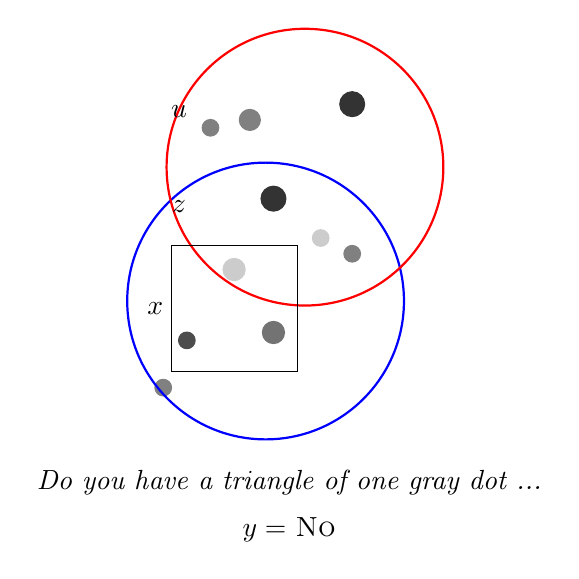
\begin{tikzpicture}

%\filldraw[gray!40] (0,0) circle (.3em);
%\filldraw[gray!100] (.25,0) circle (.38em);
%\filldraw[gray!160] (.5,0) circle (.45em);

\filldraw[gray!160] (-.2,.6) circle (.45em); % 76
\filldraw[gray!40] (-.7,-.3) circle (.4em); % 51
\filldraw[gray!40] (.4,.1) circle (.3em); % 52
\filldraw[gray!100] (.8,-.1) circle (.3em); % 66

% left
\filldraw[gray!140] (-1.3,-1.2) circle (.3em); % 13
\filldraw[gray!100] (-1.6,-1.8) circle (.3em); % 14
\filldraw[gray!110] (-.2,-1.1) circle (.4em); % 74

% right
\filldraw[gray!100] (-1,1.5) circle (.3em); % 28
\filldraw[gray!100] (-.5,1.6) circle (.38em); % 69
\filldraw[gray!160] (.8,1.8) circle (.45em); % 26

% agent plans 76
% \node[
%     draw,circle,dashed,blue,thick, minimum size=1.2em,
%     %label= left:$x$
% ] (x) at (-.2,.6) {};
% % m label
% % \filldraw[gray!40] (.4,.5) circle (.3em); % 52
% \node[
%     draw,circle,dashed,red,thick, minimum size=.6em,
%     %label=left:$m$
% ] (m) at (.4,.1) {};

\draw[blue,thick] (-.3,-.7) circle (5em);
\draw[red,thick] (.2,1) circle (5em);

% s label
\draw[draw=black] (-1.5,-1.6) rectangle (0.1,0);
%\node (s) at (-.8,1) {$s$};

% u label
% \draw[draw=black] (-1.2,1.3) rectangle (1.1,2.1);
%\node (u) at (-1.05,1.95) {$u$};
\node (u) at (-1.4, 1.7) {$u$};
\node (s) at (-1.4,0.5) {$z$};
% z label
%\node (z) at (-2.7,1) {$z$};
% d label
\node (d) at (-2.7,-.7) {$\mcD$};
\node (x) at (-1.7,-0.8) {$x$};
 
% \node (xe) at (-3.23,-3) {$x=$};
%\filldraw[gray!40] (-2.5,-3) circle (.3em); % 52
% \filldraw[gray!160] (-2.5,-3) circle (.45em); % 76
% \draw[dashed,blue,thick] (-2.5,-3) circle (.6em);

\node (v) at (-0, -3) {\textit{Do you have a triangle of one  gray dot ... }};

\node (y) at (-0,-3.6) {$y=$ \textsc{No}};
% \node (m) at (0,-3.6) {$m=$};
% \filldraw[gray!40] (.7,-3.6) circle (.3em); % 52
% \draw[dashed,red,thick] (.7,-3.6) circle (.5em);

%\node (v) at (-0, -4.2) {$y=$ No, I don't see those.};

\end{tikzpicture}
}
\caption{In \textsc{OneCommon},
the agent's perspective $\mcD$ is represented by the large blue circle,
and the partner's unobserved perspective by the red.
The shared dots $z$ are in both perspectives,
while the unshared dots $u$ are only in the red circle. 
The agent plan $x$ is given by the dots in the box,
and also described in language.
The partner response $y$ is a binary confirmation.
}
\label{fig:xzy}
\end{figure}

\subsection{Partner model}

% There are two challenges for planning with a partner model in \textsc{OneCommon}.
% First, marginalizing over the unobserved partner perspective, $\int_z p(y,z\mid x)dz$, is intractable because the dots in $z$ have continuous-valued sizes, colors, and positions.
% % This is solved by discretization.
% We address this using feature discretization.
% Second, the number of possible discretized partner perspectives $z$ is still large.
% We make marginalization tractable by decomposing the partner perspective $z$ into wo components: dots which are shared and unshared with the agent, %dots which are shared and unshared with the agent,
% and constrain the partner model to reason about them separately.
% breaking down the computation of marginalization into tractable steps.

We build a partner model by factoring the shared perspective $z$ and partner response $y$ as illustrated in Figure \ref{fig:xzy}. 
Formally,
\begin{align*}
p(y \mid x) &= \sum_z p(y\mid x,z)p(z) \\
&= \sum_{z,u}  p(y \mid x, z, u)p(z)p(u),
\end{align*}
where we introduce the latent variable $u$ representing the unshared dots in the partner perspective.

The shared dot prior, $p(z)$, is a distribution over subsets of $\mcD$, indicating which dots in the agent perspective $\mcD$ are shared with the partner.
The model $p(z)$ is initially uniform over dot subsets at the start of a game,
but is updated given evidence from the partner response $y$ at the end of each turn, $p(z \mid x, y)$. For notational simplicity we focus on the first turn.

The unshared dot prior, $p(u)$, is a distribution over the remaining partner dots.
Since the dots in $u$ are unobserved by the agent, we parameterize $p(u \mid s)$ using a uniform distribution over discretized features for each dot.
We ignore spatial features for dots in $u$
and discretize the other originally continuous features: size and color.%
\footnote{
We discretize size and color uniformly into 3 buckets based on their absolute range
across \textsc{OneCommon}.
}


%\justin{optional ->}
%The support of $p(u \mid s)$ is larger than $p(s)$: for $|u| = 3$, there are $9^3 = 728$ feature combinations.

%\justin{optional ->}
% The size of the support of $p(z)$ increases multiplicatively with the size of $p(u \mid s)$, making marginalization computationally costly.
% \daniel{insert forward reference here to where you describe how you address this?}

%\noindent \textbf{Response}
% The response model,
% % $$p(y \mid x,z) = p(c \mid x,z)p(m\mid z)p(w\mid c,m),$$
% factors into unshared, confirmation, and word models.
The confirmation model, $p(y \mid x,z)$, checks whether a partner will confirm or deny the agent plan. The partner confirms if they are able to resolve the plan $x$ to their perspective. Given a fully observed $z$ and $u$, resolution of a plan $x$ is performed by matching the features of $x$ to $z$ and $u$.
There are no trained parameters in resolution, as it depends only on the features of dots in $x$, $z$, and $u$.
See Appendix \ref{sec:feature-resolution} for the details of feature-based resolution.

In order to avoid jointly enumerating $z$ and $u$, the model reasons separately about $z$ and $u$ by making the simplifying assumption that plans are fully in $z$ or $u$.
This means that the model will deny if part of $x$ is in $z$, while the remainder is in $u$ (and $x$ is not fully contained in either $z$ or $u$):
\begin{align*}
p(y=\textsc{no}\mid x) &=\sum_{z,u} p(y=\textsc{no} \mid x, z, u)p(z,u)\\
&=\sum_z p(y=\textsc{no}\mid x, z )p(z)\\
&\quad \cdot \sum_u p(y=\textsc{no}\mid  x, u )p(u).
\end{align*}
Given the unsuccessful resolution of $x$ to both $z$ and $u$, the partner denies accurately with probability $\theta$, a hyperparameter.

% The confirmation model, $p(c \mid x,z,u)$, 
% checks if the partner confirms our plan
% based on their perspective.
% We make the simplifying assumption that a confirmation,
% $c = \text{\textsc{yes}}$, indicates that a plan $x$ resolves fully to either \justin{does either imply exclusive? its not an exclusive or} $z$ or $u$.\footnote{We ignore overlaps for computational efficiency, see Appendix \ref{sec:marginal-confirmation}}.
% % This means that the partner disconfirms if part of $x$ resolves to $s$ and the remainder to $u$,
% % and there is no other way to resolve $x$ to either $s$ or $u$.
% % We demonstrate how this assumption improves the computational complexity of computing the marginal confirmation distribution
% % in Appendix \ref{sec:marginal-confirmation}.
% When considering matches to $z$ all bucketed features (size, color, and spatial position) are checked.\footnote{
% The pairwise spatial position between dots  is bucketed into four
% relations: 
% above-left, above-right, below-left, or below-right.
% }
% When considering possible matches to $u$, spatial features are ignored for efficiency.

%\noindent \textbf{Response}
%Given a successful resolution of $x$ the partner confirms with probability $\theta$.
% The same parameter $\theta$ also determines disconfirmation given unsuccessful resolution.
% \daniel{how is $\theta$ set?}


% The mention model, $p(m \mid z)$, is a distribution over
% possible partner referents, represented as subsets of $z$.
% We assume that partner referents are not split between $s$ and $u$:
% mentions $m$ are chosen by first choosing either $s$ or $u$ with equal probability, then uniformly choosing a subset of dots from either $s$ or $u$ respectively.
% % allows same distributive trick

%The utterance model, $p(y \mid c)$, is a uniform distribution over sentences that confirm or deny the plan. \srush{This part needs to actually be written.}

\subsection{Inference}
\label{sec:inference}

% In the remainder of this section, we give the specifics of inference in \textsc{OneCommon}.
% As the goal of \textsc{OneCommon} is to find a dot in common,
% The agent plans by optimizing 
% Throughout, the agent marginalizes over the uniform $p(u\mid s)$,
% a conservative assumption that all unshared dots configurations are possible.
% This causes the agent to avoid plans that are likely to be incorrectly resolved to the unshared dots regardless of any information gathered,
% resulting in richer, more specific plans.
%\daniel{Justify this better, e.g. move the text from  "Belief update" (``avoid plans... any information gathered'') here. Or, might be worth adding something to reinforce that beliefs do still update in a useful way if possible, as otherwise this may seem like a big limitation. This doesn't have to come at this point in the paper, but it could help generally to have e.g. a qualitative example showing how the belief over the observed dots changes as we get more utterances.}

During inference, we need to compute $p(y \mid x)$ for all plans $x$,
which can be done in two steps: First, we marginalize over the unshared dots $u$.
This marginalization can be expressed in closed form.
For the details, see Appendix \ref{sec:unshared-marginal}.
Second, we marginalize over the possible set of shared dots $z$.
The computational cost of marginalization is the size of the power set of $\mcD$, $O(2^{|\mcD|})$.

%\footnote{Marginalization over the unshared perspective in the partner model can be precomputed for an entire dialogue given the agent perspective $\mcD$, thanks to the specifics of the partner model parameterization. See Appendix \ref{sec:information-gain} for the details on precomputing marginal distributions for planning.}

We utilize this distribution to compute the posterior on the shared perspective $z$, after observing a partner response to a plan,
$$ p(z \mid x,y) = \frac{ p(z, y \mid x)}{p(y \mid x)}.$$
This posterior then allows us to perform optimization over plans with respect to the expected information gain, as well as update our beliefs given the partner response.

% Accounting for the unshared dots in the partner perspective in this manner encourages the agent to choose plans which are less likely to have counterparts that only the partner can see.

\noindent \textbf{Planning} Planning optimizes the expected information gain with respect to the shared perspective $z$:
$$\argmin_x \Es{y\mid x}{H(z \mid x,y)}.$$
Computing $p(y \mid x)$ has cost $O(2^{|\mcD|})$,
while there are also $O(2^{|\mcD|})$ plans.\footnote{
Plans $x$ are subsets of $\mcD$ that the agent would like to ask the partner about.
}
As a result, optimizing this objective takes $O(2^{2|\mcD|})$ computation, and is performed in less than one second on CPU.% in real-time.
% \daniel{might be a good place to say that this is still fast enough to run on a CPU in real-time, or give a forward ref to where you say that}

\textbf{Belief update}
The belief update directly uses the posterior distribution $p(z \mid x,y)$, as described in Section \ref{sec:planning}.

During gameplay in \textsc{OneCommon}, the agent either directly observes the symbolic response $y$ or receives a description of $y$ in natural language.
In order to process the natural language dialogue,
we use a classifier to extract $y$ from natural language. 
Additionally, the partner can mention dots of their own, either symbolically or described in text.
The agent incorporates partner mentions into its belief by treating them as a confirmed plan.
We use another classifier to extract partner mentions from text.
We give the details of both the response and mention classifiers in Section \ref{sec:exp}.

\textbf{Selection}
To determine when to select a dot, the agent uses a threshold on the entropy $H[z]$, given by the hyperparameter $\tau$.
The agent them communicates which dot to select by
describing the configuration of four dots with the
highest marginal probability of being shared,
as well as the dot within that configuration that is most likely to be shared.
The agent then selects the described dot.


\section{Feature-based resolution}
\label{sec:feature-resolution}
Feature-based resolution featurizes a plan $x$
then compares the features to all subsets of dots
in the partner domain $\mcD$.
The set of features used for each plan $x$ is given by the shape and size
each dot in the plan, bucketed into 3 bins based on the range of each feature.
The pairwise positions, limited to above-left, above-right, below-left, and below-right, are also contained in the feature set.
We provide an example of feature-based resolution in Figure
\ref{fig:resolution-example}.

Given a plan $x$, feature-based resolution
must compare all the features of the plan,
of which there are $O(|x|^2)$,
to all partial permutations of subsets size $|x|$ taken from $\mcD$,
of which there are $O(|\mcD|^{|x|})$.
This can be precomputed at the start of a dialogue.

When resolving $x$ to unshared dots, we ignore spatial features.

\begin{figure}[t]
\setlength{\abovecaptionskip}{0pt}

\centering

\scalebox{1.1}{
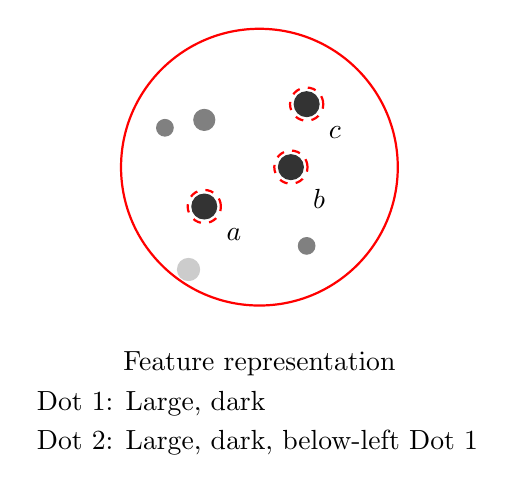
\begin{tikzpicture}


\filldraw[gray!160] (-.5,.5) circle (.45em); % 76
\filldraw[gray!40] (-.7,-.3) circle (.4em); % 51
\filldraw[gray!100] (.8,0) circle (.3em); % 66
\filldraw[gray!100] (-1,1.5) circle (.3em); % 28
\filldraw[gray!100] (-.5,1.6) circle (.38em); % 69
\filldraw[gray!160] (.8,1.8) circle (.45em); % 26
\filldraw[gray!160] (.6,1) circle (.45em); % 26

%\draw[dashed,blue,thick] (-.3,-.7) circle (5em);
\draw[red,thick] (.2,1) circle (5em);

\node[
    draw,circle,dashed,red,thick, minimum size=1.2em,
    label=below right:$a$
] (a) at (-.5,.5) {};
\node[
    draw,circle,dashed,red,thick, minimum size=1.2em,
    label=below right:$c$
] (c) at (.8,1.8) {};
\node[
    draw,circle,dashed,red,thick, minimum size=1.2em,
    label=below right:$b$
] (b) at (.6,1) {};

\node (f) at (.2, -1.5) {Feature representation};

\node[anchor=west] (f1) at (-2.75, -2) {Dot 1: Large, dark};
\node[anchor=west] (f2) at (-2.75, -2.5) {Dot 2: Large, dark, below-left Dot 1};

\end{tikzpicture}
}
\vspace{1em}
\caption{
An example of feature-based resolution.
The above feature representation for a pair of dots
resolves to dot configurations $\set{(a,b), (a,c), (b,c)}$.
}
\label{fig:resolution-example}
\end{figure}

\section{Resolution to unshared dots}
\label{sec:unshared-marginal}
The partner model, with the assumption that
$x$ cannot be split between $z$ and $u$,
is given by
\begin{align*}
&p(y=\textsc{no} \mid x)\\
&= \sum_{z,u}p(y = \textsc{no} \mid x,z,u)p(z)p(u)\\
&\approx \sum_{z,u}p(y=\textsc{no} \mid x,z)p(z) p(y=\textsc{no} \mid  x,u)p(u)\\
&= \sum_z p(y=\textsc{no} \mid x,z)p(z) \sum_u p(y=\textsc{no} \mid  x,u)p(u)\\
&= \sum_z p(y=\textsc{no} \mid x,z)p(z) \sum_u p(y=\textsc{no},u \mid  x).
\end{align*}
The probability a plan $x$ resolves to the unshared dots $u$ is
\begin{align*}
\sum_u p(y=\textsc{no},u \mid x)
&= 1-\theta {|u|\choose|x|}\frac{B^{2 \cdot (|u|-|x|)}}{B^{2\cdot|x|}},
\end{align*}
where $B$ is the feature bucket size,
given $|u| \ge |x|$.
This relies on the assumption that spatial features are ignored when resolving to unshared dots.

\section{Planning objective}
In addition to maximizing the information gain,
we also add an entropy rate constraint to the planning objective,
motivated by the entropy rate constancy and uniform information density hypotheses \citep{erc,uid,ercdial}.

In order to enforce a limit on the entropy rate, 
we limit the surprisal of the next mention proposals
under a mention model $p(x_t | x_1,\ldots,x_{t-1})$ \justin{how to include partner mentions and confirmations?}.
We could utilize the belief state $p(z = x_t)$ for this model \justin{include other history?}; however, this model is not sensitive to the ordering of plans in $h$.
We model mentions with an linearly decaying cache model,
\citep{cache}:
\begin{align*}
&p_{\text{cache}}(x_T \mid h)\\
&\propto \prod_d e^{\beta m([x_T]_d,h)
    \mathbf{1}([x_T]_d\in h)
}
e^{\alpha\mathbf{1}([x_T]_d \notin h)},
\end{align*}
where
$$m([x_T]_d,h) = T - \argmax_t t\mathbf1([x_T]_d \in h_t),$$
and $\beta$ and $\alpha$ are hyperparameters that control
the cost of unmentioned dots and recency bias respectively.

We also experiment with a supervised neural model \justin{include other history?}.

\section{Partner confusion model}
In the previous section, we introduced processing cost (as a channel capacity constraint) in the planning objective to limit the amount of information conveyed by an agent.
This is an anti-causal approach: Adding processing cost to the objective does not model the effects of a plan.
In this section we give a causal model of partner confusion as a result of processing cost.

The generative process for a response, given in Section \ref{sec:plan-oc}, is given by:
given a plan $x$, resolve that plan to the shared dots $z$ or unshared dots $u$. If the plan resolves to one or both, the partner gives a confirmation $y = \textsc{Yes}$.
Unfortunately, this partner model assumes superhuman levels of resolution.

In our human studies, we found that certain plans are difficult for humans to resolve. Plans that involve contextually vague color or size descriptors, or dots that are too far apart result in the denial of a plan that should have been confirmed.
Additionally, we believe some human players were frustrated by the information-dense descriptions of inhuman model plans, leading to poor success rates.
In this section we describe several changes to the partner model that better reflect the behaviour of a human partner.

There are three desiderata:
\begin{enumerate}
\item Spatial locality: The partner will deny a plan if the dots are too far apart
\item Channel capacity: The partner will deny a plan if there is too much new information
\item Information locality: The partner has limited memory and will treat repeated old information as new information
\end{enumerate}

We incorporate these desiderata by building them into the partner model.
We utilize a product of experts formulation,
where we combine the original partner resolution model
with a confusion model.
The goal of the confusion model is to model the effort a human partner would be willing to put into resolving a plan.
The product of experts formulation allows the confusion model to
vote against confirmation,
resulting in the response model predicting denial if the plan is theoretically resolvable, but too confusing for a human to actually understand.

Let $h$ be the history of all previous plans,
with $[h]_t = x_t$.
The full partner response model is given by
$$
p(y \mid x, z, u, h)
\propto \underbrace{p_r(y \mid x,z,u)}_{\text{resolution}}
\underbrace{p_c(y \mid x,z,h)}_{\text{confusion}}.
$$
The confusion model itself is a product of experts,
consisting of spatial and temporal confusion models:
$$
p_c(y\mid x,z,h) \propto
\underbrace{p(y \mid x,z)}_{\text{spatial}}
\underbrace{p(y \mid x,h)}_{\text{temporal}}.
$$

\subsection{Spatial model}
For the spatial model, we assume a plan is more likely to be denied if the dots in the plan are far apart.
A first approach would be to either use the distance between the furthest pair of dots, the sum of the pairwise distances between dots, or the area of the convex hull of the dots.
However, as the distances of dots may vary,
we instead use the relative rankings of dot distances.
This mimics one possible method of dot resolution, where the partner first finds an anchor dot then searches nearby to find the remaining dots in the plan.
As a result, we have
$$
p(y = \textsc{No} \mid x)
= \min_{d\in x} \frac{
\sum_{d'\in x} r(d,d')
}{
1+\sum_{i=7-|x|+1}^7 i
},
$$
where $r(d,d')$ gives the rank of dot $d'$ to $d$ in order of increasing distance given the agent's perspective.
%\justin{will fix up later}
nswer both time, and take that into account with the partner model.

\section{Supervised partner model}


\section{Selection objective}

\section{Describing plans}
The success of an agent that plans through a partner model is limited
by the accuracy of its partner model.
While the partner model predicts the partner's reaction to the agent's plan,
a human partner receives a natural language description of the agent's plan.
For the partner model to be accurate, the plan description must be precise.

Preliminary experiments indicate that a model from previous work \citep{fried}
loses precision when describing plans involving more than a single dot.
We hypothesize that this is due to data imbalance.



\end{document}

